\documentclass{beamer}

\usepackage[utf8]{inputenc}
\usepackage[T1]{fontenc}
\usepackage[english]{babel}
\usepackage{setspace}
\usepackage{color}
\usepackage{listings}
\usepackage{pgf-pie}
\usepackage{pgfplots}

\usetheme[progressbar=frametitle]{metropolis}
\setbeamertemplate{frame numbering}[fraction]
\useoutertheme{metropolis}
\useinnertheme{metropolis}
\usefonttheme{metropolis}
\usecolortheme{spruce}
\setbeamercolor{background canvas}{bg=white}

\title[Micronaut]{Introduction to Micronaut Framework}
\subtitle{A modern, JVM-based, full-stack framework for building modular, easily testable microservice and serverless applications.}
\author{\texorpdfstring{Albert Attard\newline\url{albert.attard@thoughtworks.com}}{Albert Attard}}
\institute{\large \href{https://thoughtworks.com}{\textbf{ThoughtWorks}.com}}
\date{}

\begin{document}
  \metroset{block=fill}

  \begin{frame}
    \titlepage
  \end{frame}


  \begin{frame}[t]{Micronaut}
    \textbf{What is Micronaut?}\\[6pt]
    Micronaut is a framework based on the JVM that enables fast development of low memory footprint application.

    This makes it a good candidate for building microservices and serverless applications.
  \end{frame}

  \begin{frame}[t]{Another Framework?}
    \textbf{Spring Boot} dominates the market, according to \href{https://www.jrebel.com/sites/rebel/files/pdfs/ebook-jrebel-java-productivity-report.pdf}{JRebel's 2020 Java Developer Productivity Report}

    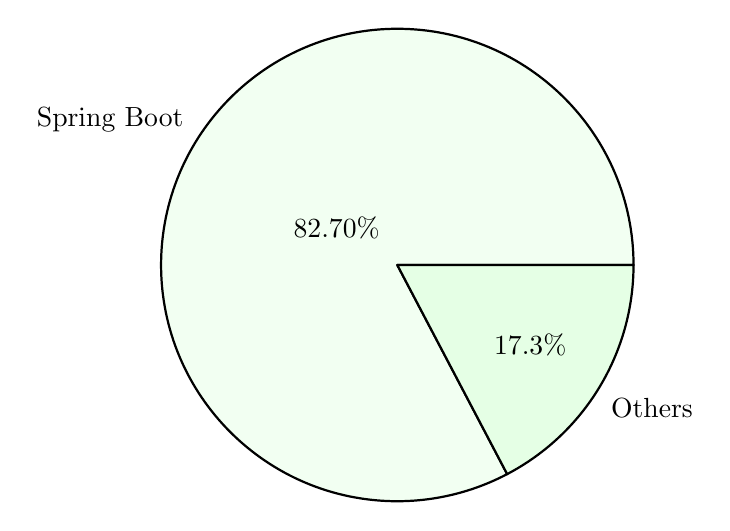
\begin{tikzpicture}
      \pie [rotate = 0, color={green!5, green!10}]
      {82.70/Spring Boot,
      17.3/Others}
    \end{tikzpicture}

  \end{frame}


  \begin{frame}[t]{Spring Boot}
    Spring Boot is a sold framework that leverages the Spring ecosystem and enables fast development cycles and minimise boilerplate

    It simplifies bootstrapping and development of new Spring based applications by providing opinionated defaults.

    Spring Boot provides a vast number of libraries that take advantage of it and make is easy to adopt (\href{https://docs.spring.io/spring-boot/docs/2.0.0.M5/reference/html/boot-features-developing-auto-configuration.html}{using the auto-configuration}).

    \vspace{16pt}
    \textbf{So why don't we use Spring Boot?}
  \end{frame}


  \begin{frame}[t]{Reflection}
    Spring, like many other libraries, rely on reflection to resolve dependencies and perform key tasks

    Reflection has two main drawbacks
    \begin{itemize}
      \item \textbf{Memory} - each library that makes use of reflection creates its own cache, with the class being the smallest unit.
      \item \textbf{Performance} - the application need to perform all reflection logic at runtime which slows the application down
    \end{itemize}

    \vspace{16pt}
    Spring Boot enables fast development, but suffers from slow start-up time and higher memory footprint
  \end{frame}


  \begin{frame}[t,fragile]{Why do we need Reflection?}
    Spring Boot, relies on annotations to work

    Take for an instance the following bean definition

    \vspace{16pt}
    \begin{lstlisting}[language=Java, backgroundcolor = \color{green!5}]
@Bean
fun runner() =
  CommandLineRunner {}
    \end{lstlisting}

    \vspace{16pt}
    Spring Boot will scan our project search for beans and it needs reflection to do this
  \end{frame}


  \begin{frame}[t]{Using the Compiler}
    Micronaut takes a different approach
    \begin{itemize}
      \item \textbf{Compiler} - resolves as much as possible at compile time
      \item \textbf{Reflection} - minimise the usage of reflection
      \item \textbf{Productive} - make use of Spring like annotations, to keep productivity up
    \end{itemize}
  \end{frame}


  \begin{frame}[t]{Memory Footprint}
    \begin{center}
      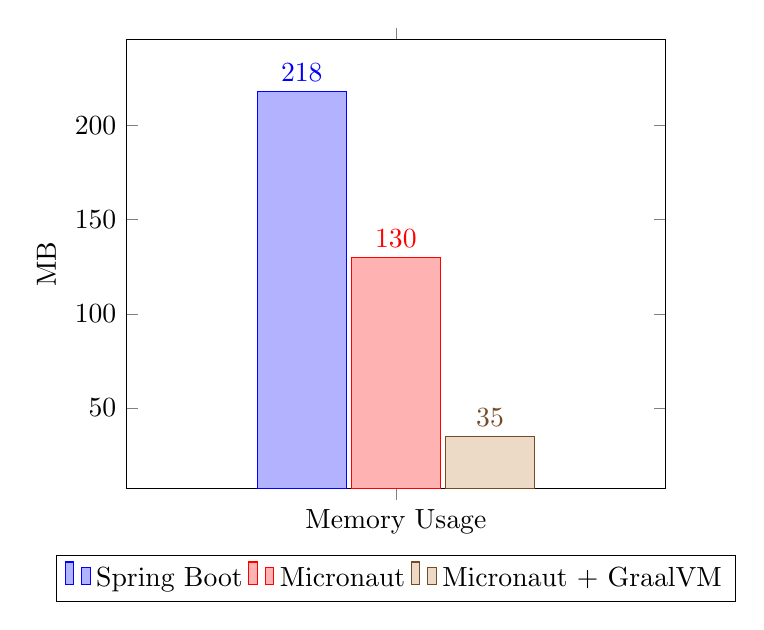
\begin{tikzpicture}
        \begin{axis}[
          ybar,
          bar width=32pt,
          enlargelimits=0.15,
          legend style={at={(0.5,-0.15)},
          anchor=north,legend columns=-1},
          ylabel={MB},
          symbolic x coords={Memory Usage},
          xtick=data,
          nodes near coords,
          nodes near coords align={vertical},
        ]
          \addplot coordinates {(Memory Usage,218)};
          \addplot coordinates {(Memory Usage,130)};
          \addplot coordinates {(Memory Usage,35)};
          \legend{Spring Boot,Micronaut,Micronaut + GraalVM}
        \end{axis}
      \end{tikzpicture}
    \end{center}
  \end{frame}


  \begin{frame}[t]{Time to First Response}
    \begin{center}
      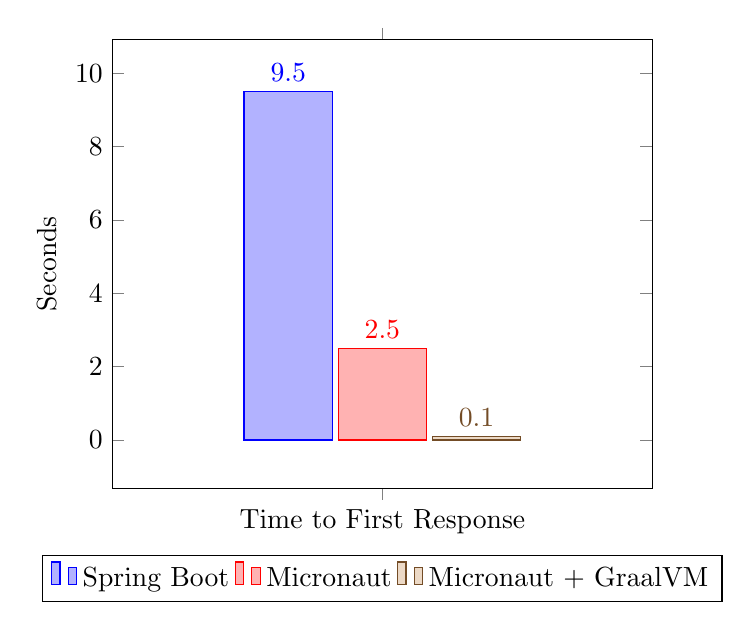
\begin{tikzpicture}
        \begin{axis}[
          ybar,
          bar width=32pt,
          enlargelimits=0.15,
          legend style={at={(0.5,-0.15)},
          anchor=north,legend columns=-1},
          ylabel={Seconds},
          symbolic x coords={Time to First Response},
          xtick=data,
          nodes near coords,
          nodes near coords align={vertical},
        ]
          \addplot coordinates {(Time to First Response, 9.5)};
          \addplot coordinates {(Time to First Response, 2.5)};
          \addplot coordinates {(Time to First Response, 0.1)};
          \legend{Spring Boot,Micronaut,Micronaut + GraalVM}
        \end{axis}
      \end{tikzpicture}
    \end{center}
  \end{frame}


  \begin{frame}[t]{using Blocks}
    \begin{block}{Micronaut}
      \textbf{Micronaut} is a modern, JVM-based, full-stack framework for building modular, easily testable microservice and serverless applications
    \end{block}
  \end{frame}

\end{document}
